
\chapter{Thiết kế cơ sở dữ liệu}
\label{chap:db}

\section{Mô hình ERD}
\begin{figure}[H]
\centering
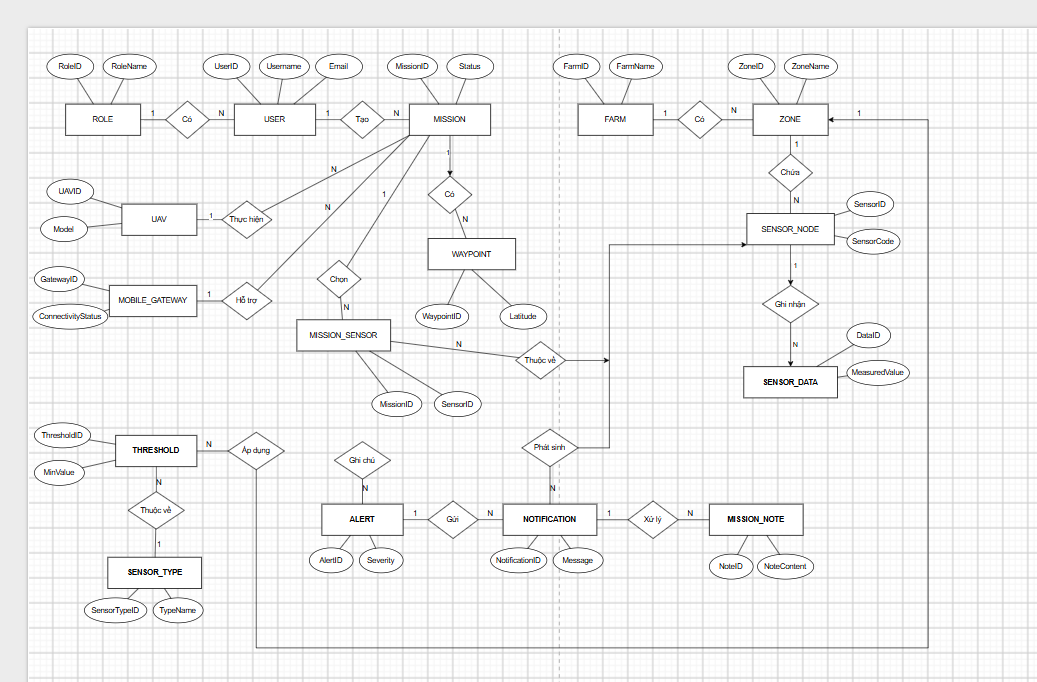
\includegraphics[width=\textwidth,height=0.76\textheight,keepaspectratio]{figures/erd_tong_quan.png}
\caption{ERD tổng quan}
\label{fig:erd}
\end{figure}

Hình trên là sơ đồ ERD tổng quan mà. Các entity bao phủ role/user, farm/zone, mission/UAV/gateway, sensor node/sensor data, threshold, alert và notification.

\section{Các nhóm bảng}
\begin{longtable}{p{4cm}p{9.5cm}}
\caption{Phân nhóm bảng trong thiết kế}\label{tab:tablegroups}\\
\toprule
Nhóm & Bảng \\
\midrule
Identity & ROLE, USER\\
Farm & FARM, ZONE\\
Sensor & SENSOR\_TYPE, SENSOR\_NODE, SENSOR\_DATA, THRESHOLD\\
UAV & UAV, MOBILE\_GATEWAY\\
Mission & MISSION, MISSION\_SENSOR, WAYPOINT, MISSION\_COLLECTION, MISSION\_NOTE\\
Alert & ALERT, NOTIFICATION, ALERT\_HANDLING\\
\bottomrule
\end{longtable}

\section{Lược đồ quan hệ}
Các ảnh schema chi tiết được đưa vào báo cáo ở Phụ lục. Các bảng và cột dưới đây được mô tả theo sơ đồ thiết kế.

\begin{longtable}{p{3.5cm}p{10cm}}
\caption{Danh mục bảng và mục đích}\label{tab:dictionary}\\
\toprule
Bảng & Mục đích \\
\midrule
ROLE & Danh mục vai trò người dùng.\\
USER & Tài khoản, thông tin đăng nhập và trạng thái người dùng.\\
FARM & Thông tin nông trại.\\
ZONE & Khu vực thuộc farm.\\
SENSOR\_NODE & Thiết bị cảm biến được đăng ký tại zone.\\
SENSOR\_TYPE & Loại chỉ số cảm biến và đơn vị đo.\\
SENSOR\_DATA & Measurement theo sensor node và sensor type.\\
THRESHOLD & Ngưỡng kiểm tra theo sensor type/zone.\\
UAV & Thiết bị bay được quản lý trong hệ thống.\\
MOBILE\_GATEWAY & Gateway gắn với UAV, phục vụ collection/sync.\\
MISSION & Nhiệm vụ thu thập dữ liệu.\\
MISSION\_SENSOR & Bảng liên kết mission--sensor.\\
WAYPOINT & Các điểm tuyến bay của mission.\\
MISSION\_COLLECTION & Nhật ký từng lần thu thập, retry và lỗi.\\
MISSION\_NOTE & Ghi chú của người dùng cho mission.\\
ALERT & Cảnh báo phát sinh từ sensor data.\\
NOTIFICATION & Thông báo gửi cho user.\\
ALERT\_HANDLING & Nhật ký xử lý alert.\\
\bottomrule
\end{longtable}

\section{Quan hệ và lực lượng kết hợp}
\begin{longtable}{p{4cm}p{2cm}p{7cm}}
\caption{Các quan hệ chính}\label{tab:relations}\\
\toprule
Cha & Cardinality & Con \\
\midrule
ROLE & 1:N & USER\\
FARM & 1:N & ZONE\\
ZONE & 1:N & SENSOR\_NODE\\
SENSOR\_NODE & 1:N & SENSOR\_DATA\\
SENSOR\_TYPE & 1:N & SENSOR\_DATA\\
SENSOR\_TYPE & 1:N & THRESHOLD\\
ZONE & 1:N & THRESHOLD\\
FARM & 1:N & UAV\\
UAV & 1:N & MOBILE\_GATEWAY\\
FARM & 1:N & MISSION\\
UAV & 1:N & MISSION\\
MOBILE\_GATEWAY & 1:N & MISSION\\
USER & 1:N & MISSION\\
MISSION & 1:N & WAYPOINT\\
MISSION & N:M & SENSOR\_NODE qua MISSION\_SENSOR\\
MISSION & 1:N & MISSION\_COLLECTION\\
SENSOR\_NODE & 1:N & MISSION\_COLLECTION\\
SENSOR\_NODE & 1:N & ALERT\\
ALERT & 1:N & NOTIFICATION\\
USER & 1:N & NOTIFICATION\\
ALERT & 1:N & ALERT\_HANDLING\\
USER & 1:N & ALERT\_HANDLING\\
MISSION & 1:N & MISSION\_NOTE\\
USER & 1:N & MISSION\_NOTE\\
\bottomrule
\end{longtable}

\section{Khóa chính và khóa ngoại}
Nguyên tắc chính:
\begin{itemize}
  \item Mỗi entity chính có khóa chính định danh dạng \code{VARCHAR(20)} theo sơ đồ.
  \item Khóa ngoại dùng cùng kiểu với khóa được tham chiếu.
  \item \code{MISSION\_SENSOR} dùng khóa ghép gồm \code{MissionID} và \code{SensorID}.
  \item Các quan hệ 1:N được triển khai bằng FK ở phía N.
  \item Quan hệ N:M giữa mission và sensor node được chuẩn hóa bằng bảng trung gian.
\end{itemize}

\section{Chuẩn hóa và toàn vẹn dữ liệu}
Thiết kế tách riêng farm, zone, sensor type, sensor node và sensor data giúp giảm lặp dữ liệu. Các thuộc tính mô tả entity không cần lặp lại trong bảng measurement. Tương tự, threshold được tách khỏi sensor data để thay đổi cấu hình mà không phải cập nhật lịch sử measurement.

Các constraint nên được áp dụng ở mức database:
\begin{itemize}
  \item \code{PRIMARY KEY} cho mọi bảng.
  \item \code{FOREIGN KEY} cho các quan hệ.
  \item \code{UNIQUE} cho các mã nghiệp vụ như username, email, sensor code, serial number nếu quy tắc nghiệp vụ xác nhận tính duy nhất.
  \item \code{NOT NULL} cho các cột bắt buộc.
  \item \code{CHECK} cho các giá trị số như battery level trong khoảng hợp lệ và MinValue $\le$ MaxValue.
\end{itemize}

\section{Index đề xuất}
Để đáp ứng truy vấn dashboard và collection:
\begin{itemize}
  \item index \code{SENSOR\_DATA(SensorID, MeasuredAt)};
  \item index \code{SENSOR\_DATA(SensorTypeID, MeasuredAt)};
  \item index \code{MISSION\_COLLECTION(MissionID, Status)};
  \item index \code{ALERT(SensorID, Status, TriggeredAt)};
  \item index \code{NOTIFICATION(UserID, Status, SentAt)};
  \item index \code{WAYPOINT(MissionID, SequenceNo)}.
\end{itemize}

\section{Hình schema chi tiết}
Các sơ đồ schema được tích hợp trong Phụ lục. Chúng được chia theo các cụm: user/farm/zone; sensor/threshold; UAV/mission; collection/alert.
